\thispagestyle{empty}\SourceLeaf{002}
\vspace*{1in}
\begin{center}
{\Large\bfseries CARL FRIEDRICH GAUSS WERKE\par}
\vspace{.45in}
{\large\bfseries BAND IV.\par}
\end{center}
\clearpage
\thispagestyle{empty}\SourceLeaf{004}
\begin{center}
{\Large\bfseries CARL FRIEDRICH GAUSS\par}
\vspace{.25in}
{\Huge\bfseries WERKE\par}
\vspace{.3in}
{\large\bfseries VIERTER BAND.\par}
\vspace{.4in}
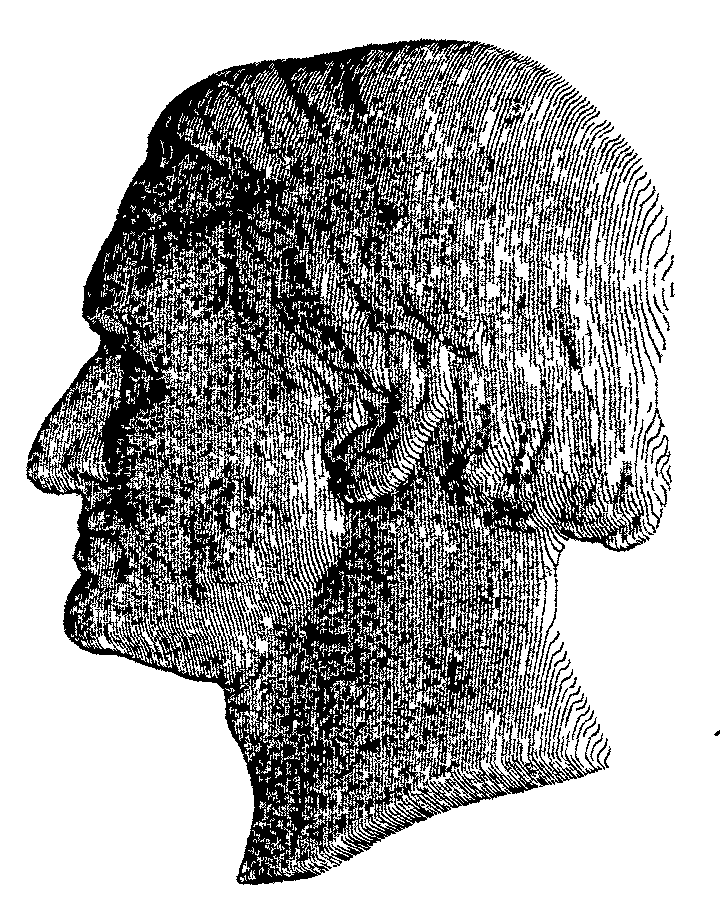
\includegraphics[height=2.45in]{assets/native004_original_portrait.png}
\vspace{.4in}

{\small HERAUSGEGEBEN\par}
\medskip
{\small VON DER\par}
\medskip
{\normalsize KÖNIGLICHEN GESELLSCHAFT DER WISSENSCHAFTEN\par}
\smallskip
{\small ZU\par}
\medskip
{\large GÖTTINGEN\par}
\smallskip
1873.
\end{center}
\clearpage
\thispagestyle{empty}\SourceLeaf{006}
\begin{center}
\vspace*{.25in}
{\Large THEORIE\par}
\vspace{.3in}
{\Large\bfseries DER KOMBINATION VON BEOBACHTUNGEN\par}
\vspace{.2in}
{\large DIE DEN KLEINSTEN FEHLERN AUSGESETZT IST\par}
\vspace{.4in}
{\large ERSTER TEIL\par}
\vspace{.45in}
{\small VON\par}
\vspace{.3in}
{\large CARL FRIEDRICH GAUSS\par}
\vspace{.45in}
{\small DER KÖNIGLICHEN GESELLSCHAFT DER WISSENSCHAFTEN VORGELEGT 1821. FEBR. 15.\par}
\vspace{.4in}
\rule{.9\linewidth}{.3pt}\par
\smallskip
{\small Commentationes societatis regiae scientiarum Gottingensis recentiores. Vol.\,v.\par}
\smallskip
{\small Göttingen \textsc{mdcccxxiii}.\par}
\smallskip
\rule{.9\linewidth}{.3pt}
\end{center}
\clearpage
\SourceLeaf{008}
\begin{center}
{\large THEORIE\par}
\medskip
{\Large\bfseries DER KOMBINATION VON BEOBACHTUNGEN\par}
\medskip
{\large DIE DEN KLEINSTEN FEHLERN AUSGESETZT IST.\par}
\medskip
{\large\textsc{Erster Teil.}\par}
\medskip
\rule{.22\linewidth}{.3pt}
\end{center}
\Article{1}
Mit wie großer Sorgfalt auch Beobachtungen angestellt werden, die sich auf die Größe natürlicher Dinge beziehen, bleiben sie doch stets größeren oder kleineren Fehlern ausgesetzt. Beobachtungsfehler sind meistens nicht einfach, sondern entspringen zugleich mehreren Quellen: Zwei Arten dieser Quellen müssen sorgfältig unterschieden werden. Manche Fehlerursachen sind so beschaffen, dass ihre Wirkung bei jeder Beobachtung von veränderlichen Umständen abhängt, zwischen denen und der Beobachtung selbst kein wesentlicher Zusammenhang angenommen wird: Die daraus entstehenden Fehler heißen unregelmäßige oder zufällige Fehler, und soweit jene Umstände keiner Berechnung unterworfen werden können, gilt dasselbe auch für die Fehler selbst. Hierher gehören die Fehler, die aus der Unvollkommenheit der Sinne entstehen, ebenso wie diejenigen aus unregelmäßigen äußeren Ursachen, z. B. aus der zitternden Bewegung der Luft, die das Sehen ein wenig stört: Auch mehrere Mängel selbst der besten Instrumente sind hierher zu rechnen, z. B. die Rauheit im Inneren der Wasserwaagen, das Fehlen absoluter Festigkeit usw. Andere Fehlerursachen dagegen üben ihrer Natur nach bei allen Beobachtungen derselben Art eine Wirkung aus, die entweder absolut konstant ist oder wenigstens eine Größe hat, die nach einem bestimmten Gesetz allein von Umständen abhängt, welche als wesentlich mit der Beobachtung verbunden angesehen werden. Derartige Fehler heißen konstante oder regelmäßige Fehler.

Im Übrigen ist offensichtlich, dass diese Unterscheidung in gewissem Maße relativ ist und davon abhängt, ob der Begriff der Beobachtungen derselben Art in einem weiteren oder engeren Sinn genommen wird. So erzeugen z. B. unregelmäßige Mängel in der Teilung von Instrumenten zur Messung von \SourceLeaf{009}Winkeln einen konstanten Fehler, wenn es lediglich um die beliebig oft zu wiederholende Beobachtung eines bestimmten Winkels geht, da hierbei immer dieselben fehlerhaften Teilstriche benutzt werden: Dagegen kann der aus jener Quelle entstehende Fehler als zufällig angesehen werden, wenn es ohne nähere Bestimmung um die Messung von Winkeln beliebiger Größe geht, sofern keine Tabelle vorliegt, welche die Größe des Fehlers bei den einzelnen Teilstrichen angibt.

\Article{2}
Die Betrachtung regelmäßiger Fehler ist eigentlich von unserem Vorhaben ausgeschlossen. Es ist nämlich die Aufgabe des Beobachters, alle Ursachen, die konstante Fehler erzeugen können, sorgfältig zu untersuchen und entweder zu beseitigen oder wenigstens ihre Beschaffenheit und Größe mit größtem Eifer zu erforschen, damit ihre Wirkung bei jeder bestimmten Beobachtung angegeben werden kann. Die Beobachtung kann somit von dieser Wirkung befreit werden, womit es auf dasselbe hinausläuft, als wäre der Fehler überhaupt nicht vorhanden gewesen. Ganz anders verhält es sich jedoch mit den unregelmäßigen Fehlern, die ihrer Natur nach keiner Berechnung unterworfen werden können. Diese muss man daher bei den Beobachtungen zwar hinnehmen, ihre Wirkung auf die aus den Beobachtungen abzuleitenden Größen aber durch eine geschickte Kombination der Beobachtungen so weit wie möglich vermindern. Diesem höchst wichtigen Gegenstand sind die folgenden Untersuchungen gewidmet.

\Article{3}
Die Fehler bei Beobachtungen derselben Art, die aus einer bestimmten einfachen Ursache entstehen, sind der Natur der Sache nach in gewisse \textit{Grenzen} eingeschlossen, die sich zweifellos genau angeben ließen, wenn die Beschaffenheit der Ursache selbst \textit{vollständig} durchschaut wäre. Die meisten Ursachen zufälliger Fehler sind so beschaffen, dass nach dem Gesetz der Stetigkeit alle innerhalb jener Grenzen liegenden Fehler als möglich gelten müssen, und eine vollkommene Kenntnis der Ursache würde auch lehren, ob alle diese Fehler gleich wahrscheinlich oder ungleich wahrscheinlich sind. Im letzteren Fall würde sie außerdem lehren, welche relative Wahrscheinlichkeit jedem Fehler zuzuschreiben ist. Dasselbe wird auch für den aus mehreren einfachen Fehlern zusammengesetzten Gesamtfehler gelten: Er wird nämlich in gewisse Grenzen eingeschlossen sein, (deren eine gleich der Summe aller oberen Teilgrenzen, die andere gleich der Summe aller unteren Grenzen sein wird); alle Fehler innerhalb dieser Grenzen werden zwar möglich sein, doch da jeder sich auf unendlich viele verschiedene Arten aus Teilfehlern zusammensetzen lässt, die selbst mehr oder weniger wahrscheinlich sind, werden wir dem einen eine größere, dem anderen eine kleinere Wahrscheinlichkeit zuschreiben müssen, und das Gesetz der rela\SourceLeaf{010}%
tiven Wahrscheinlichkeit wird sich ermitteln lassen, wenn die Gesetze der einfachen Fehler als bekannt vorausgesetzt werden, vorbehaltlich der analytischen Schwierigkeiten beim Zusammenfassen aller Kombinationen.

Es gibt allerdings einige Fehlerursachen, die nur diskrete Fehler und keine nach dem Gesetz der Stetigkeit fortschreitenden Fehler hervorbringen können, wie etwa die Teilungsfehler der Instrumente, (wenn man sie zu den zufälligen Fehlern rechnen will): Denn die Anzahl der Teilstriche ist bei jedem bestimmten Instrument endlich. Dennoch ist offensichtlich, dass, sofern nicht alle Fehlerursachen diskrete Fehler erzeugen, die Gesamtheit aller möglichen Gesamtfehler eine nach dem Gesetz der Stetigkeit fortschreitende Reihe oder mehrere solche unterbrochenen Reihen bilden wird, falls, nachdem alle möglichen diskreten Fehler der Größe nach geordnet sind, der eine oder andere Unterschied zwischen zwei benachbarten Gliedern größer ausfällt als der Unterschied zwischen den Grenzen der Gesamtfehler, soweit diese allein aus stetigen Fehlern hervorgehen. In der Praxis wird der letztere Fall jedoch kaum jemals eintreten, es sei denn, die Teilung leidet an gröberen Mängeln.

\clearpage
